\subsection{Models and Analytics} \label{s:models}
Once the data is available and programmatically accessible through well-defined APIs, modeling types that users can perform can be considered.

Object associations can be definitive or manufactured through a probabilistic generative model to guide inference from incomplete data.  The former can be prescribed by the user by linking objects through a GUI or template; the latter through Bayesian inference \cite{Pearl:1988:PRI:52121}, which provides a rational framework for updating beliefs about latent variables in generative models given observed data \cite{MacKay:2002:ITI:971143}.

Creating Bayesian models through graphs and predicate logic is more commonly the domain of data scientists than IT users. However, the goal for our system isn't to mandate a specific model of relation (definitive or derived), but rather to take care in design to not implicitly restrict the user to a particular model. Our system must provide the flexibility to persist and mutate object relation to meet a variety of user requirements\footnote{Nate Silver discusses the breadth of problems to which Bayesian reasoning can be applied in \cite{silver2012signal}.}.

As such, our goal is to provide an abstract framework over which schemas can be applied with sufficient flexibility to allow these relations to span the prosaic, e.g. linking monotonically increasing instances of an object (creating a version tree), to the expressive, e.g. a graph schema where nodes represent variables and directed edges between nodes represent probabilistic causal links.

For example, in an epidemiology study nodes might represent whether a patient has a cold, a cough, a fever or other conditions, and the presence or absence of links indicates that colds tend to cause coughing and sinus inflammation but not fever; sinus inflammation tends to cause headache but not fever; and so on \cite{tenenbaum2011grow}. The probability of a causal relation can be further refined by applying a weighting (0 - 1.0) to each link; e.g. there's a 60\% likelihood that a cold will result in a cough. As depicted in Figure \ref{fig:epi} graphs provide a ready means for users to interpret data and visualize relationships.

\begin{figure}[h]
  \centering
    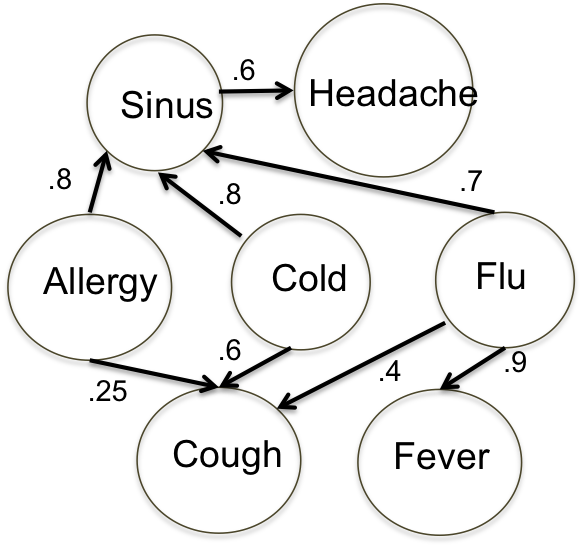
\includegraphics[width=0.3\textwidth]{fig/disease-graph.png}
  \caption{Epidemiology Directed Graph}
  \label{fig:epi}
\end{figure}

Through the proper application of multi-predicate constraints over the field of objects in a domain, the user is able to resolve to \emph{classes} of objects---such as all objects associated with the progenitor of a disease. For example a user might want to view all outcomes for patients over 60 in Africa with diminished respiratory function in the presence of the bacteria Legionella, and contrast this to those in the presence of the virus adenovirus to determine whether better outcomes are seen in patients with bacterial versus viral pneumonia.

Such analytic questions can be compute intensive when run over the full mass of \ud{} (what we refer to as \emph{data objects} in \S\ref{s:obj}), but are comparatively lightweight operations when run against the much smaller set of \md{} associated with these data objects. Here the \md{} acts an abbreviation of the objects and allows us to create information from an otherwise undistinguished data mass.
